% !TEX TS-program = pdflatex
% !TEX encoding = UTF-8 Unicode

% This is a simple template for a LaTeX document using the "article" class.
% See "book", "report", "letter" for other types of document.

\documentclass[11pt]{article} % use larger type; default would be 10pt

\usepackage[utf8]{inputenc} % set input encoding (not needed with XeLaTeX)

%%% Examples of Article customizations
% These packages are optional, depending whether you want the features they provide.
% See the LaTeX Companion or other references for full information.

%%% PAGE DIMENSIONS
\usepackage{geometry} % to change the page dimensions
\geometry{a4paper} % or letterpaper (US) or a5paper or....
% \geometry{margin=2in} % for example, change the margins to 2 inches all round
% \geometry{landscape} % set up the page for landscape
%   read geometry.pdf for detailed page layout information

\usepackage{graphicx} % support the \includegraphics command and options

% \usepackage[parfill]{parskip} % Activate to begin paragraphs with an empty line rather than an indent

%%% PACKAGES
\usepackage{booktabs} % for much better looking tables
\usepackage{array} % for better arrays (eg matrices) in maths
\usepackage{paralist} % very flexible & customisable lists (eg. enumerate/itemize, etc.)
\usepackage{verbatim} % adds environment for commenting out blocks of text & for better verbatim
\usepackage{subfig} % make it possible to include more than one captioned figure/table in a single float
% These packages are all incorporated in the memoir class to one degree or another...


%%% HEADERS & FOOTERS
\usepackage{fancyhdr} % This should be set AFTER setting up the page geometry
\pagestyle{fancy} % options: empty , plain , fancy
\renewcommand{\headrulewidth}{0pt} % customise the layout...
\lhead{}\chead{}\rhead{}
\lfoot{}\cfoot{\thepage}\rfoot{}

%%% SECTION TITLE APPEARANCE
\usepackage{sectsty}
\allsectionsfont{\sffamily\mdseries\upshape} % (See the fntguide.pdf for font help)
% (This matches ConTeXt defaults)

\usepackage{amssymb}
\usepackage{float}
%\usepackage{soul}

%%% ToC (table of contents) APPEARANCE
\usepackage[nottoc,notlof,notlot]{tocbibind} % Put the bibliography in the ToC
\usepackage[titles,subfigure]{tocloft} % Alter the style of the Table of Contents
\renewcommand{\cftsecfont}{\rmfamily\mdseries\upshape}
\renewcommand{\cftsecpagefont}{\rmfamily\mdseries\upshape} % No bold!

\usepackage{pdfpages}

%%% END Article customizations

%%% The "real" document content comes below...
\title{Work Information}
\author{Logan Brown}
%\date{} % Activate to display a given date or no date (if empty),
         % otherwise the current date is printed 

\begin{document}
\maketitle
\tableofcontents

\newpage

\section{PSUADE}

\subsection{Installing PSUADE}

\subsubsection{General Steps}

\begin{enumerate}
\item tar xzvf PSUADE.tar.gz
\item cd PSUADE\_1.7.2
\item mkdir build; cd build
\item cmake .. \&$>$ cmake.output \&

(This step will take a minute or so.)

\item make \&$>$ make.output \&

(This step will take some time.)
\end{enumerate}

If the make is successful, build/bin should contain the psuade executable. Set \$PATH and \$LD\_LIBRARY\_PATH, based on your installation location. To test your build, change to your build directory and type ``make test".


\subsubsection{Installing on Darter}

\begin{enumerate}
\item \textit{tar xzvf PSUADE.tar.gz}
\item \textit{cd PSUADE\_1.7.2}
\item \textit{mkdir build; cd build}
\item \textit{cmake ..} \&$>$ \textit{cmake.output} \&
\item {\bfseries Go to cmake\_install.cmake and change CMAKE\_INSTALL\_PREFIX from ``/usr/local/" to a directory where you have permission. }

I used ``PSUADE\_v1.7.2/inst/"

\item \textit{make} \&$>$ \textit{make.output} \&
\end{enumerate}

\subsubsection{Installing on star1}

Note: Requires cmake, you may have to install a local copy.

\begin{enumerate}
\item \textit{tar xzvf PSUADE.tar.gz}
\item \textit{cd PSUADE\_1.7.2}
\item \textit{mkdir build; cd build}
\item {\bfseries export LD\_LIBRARY\_PATH=}

~~~~{\bfseries /home/kwong/LAPACK/lib-shared/:\$LD\_LIBRARY\_PATH}

Alternatively, use another libblas.so, if you have one.
\item \textit{cmake ..} \&$>$ \textit{cmake.output} \&
\item {\bfseries Go to cmake\_install.cmake and change CMAKE\_INSTALL\_PREFIX from ``/usr/local/" to a directory where you have permission.}
\item {\bfseries Go to CMakeCache.txt and change LAPACK\_lapack\_LIBRARY:FILEPATH to}
		
~~~~{\bfseries /home/kwong/LAPACK/lib-shared/liblapack.so}

OR

~~~~{\bfseries /home/lbrown/iel-2.0/EXTLIB/LAPACK/lapack-3.4.0-shared/liblapack.so}

or to whatever liblapack.so you prefer

\item \textit{make} \&$>$ \textit{make.output} \&
\end{enumerate}


%%\newpage

\subsection{Compiling PSUADE as a Module}
\subsubsection{main in Psuade.cpp as a module}


I recommend first copying over Psuade.cpp to PsuadeIEL.cpp, and making all of the relevant changes in that file. That way, you can still compile Psuade as a standalone software piece for data analysis and debugging, in addition to compliling the Psuade module library.

If you choose to just modify Psuade.cpp, replace all instances of 'PsuadeIEL.cpp' below with 'Psuade.cpp'. The resulting library will be incapable of running PSUADE without the DIEL, because it will lack a main function.

\begin{enumerate}

	\item Add include files to PsuadeIEL.cpp

\begin{verbatim}
#include "../../../../iel-2.0/EXECUTIVE/HYBRID/IEL_comm/IEL.h"
#include "../../../../iel-2.0/EXECUTIVE/HYBRID/executive/IEL_exec_info.h"
#include "../../../../iel-2.0/EXECUTIVE/HYBRID/IEL_comm/tuple_comm.h"
#include "../../../../iel-2.0/EXECUTIVE/HYBRID/IEL_comm/arrayList.h"
\end{verbatim}


	\item Change main(int argc, char** argv)  to PSUADEmain(IEL\_exec\_info\_t *exec\_info)

%%	\item In Makefile.in, add to the end of PSUADE\_INCLUDE = -I\$(PSUADE\_DIR) -I\$(PSUADE\_DIR)/Include
%%	
%%~~~~ -I../../../../iel-2.0/EXECUTIVE/HYBRID/executive/
%%
%%~~~~ -I../../../../iel-2.0/EXECUTIVE/HYBRID/IEL\_comm/
%5
%%	\item When I initially call the CMAKE, I set the library path (to avoid catching user/bin/liblapack.so) and CMAKE\_CXX\_FLAGS to -DMPICH\_SKIP\_MPICXX
%%
%%	-DCMAKE\_LIBRARY\_PATH=\$(IEL\_HOME)/EXTLIB/LAPACK/lapack-3.4.0-shared/\\
%%	and
%%
%%	-DCMAKE\_CXX\_FLAGS='-DMPICH\_SKIP\_MPICXX'

	\item Add the following lines to CMakeLists.txt
\begin{verbatim}
SET(CMAKE_CXX_FLAGS "-DMPICH_SKIP_MPICXX")

include_directories("../../../EXECUTIVE/HYBRID/executive/")
include_directories("../../../EXECUTIVE/HYBRID/IEL_comm/")
include_directories("../../MPICH/mpich-shared/include/")
add_library (PsuadeModule ${LIBRARY_TYPE} "Src/Main/PsuadeIEL.cpp" ${psuade_SRC}
    ${psuade_HDRS} ${PDF_SRC})
\end{verbatim}

(The add\_library command should be one line, but text wrapping makes it look like two   )

\end{enumerate}

\subsubsection{Passing command line arguments to PSUADE}

Command line arguments should be passed through the argument by the cfg file.

I added these lines to the PsuadeIEL.cpp file to get the arguments. PSUADE assumes that the first argument in argv is ``/path/to/psuade/psuade", so we put a filler argument in argv[0].

\begin{verbatim}
int argc = exec_info->modules[exec_info->module_num].mod_argc + 1;

char* argv[argc];
char* temporary = "PsuadeModule";
argv[0] = temporary;
int i=0;
for(i=0; i<(argc-1); i++)
    {    argv[i+1] = exec_info->modules[exec_info->module_num].mod_argv[i];    }
\end{verbatim}



%%\newpage

PSUADE has four major functions - Sensitivity Analysis, Uncertainty Quantification, Optimization, and Data Analysis.

In general, PSUADE provides inputs to a simulation and compares it to the outputs from the simulation. It stores all of these results in a file, by default called psuadeData, which has all of the information about the inputs and the outputs. Generally, PSUADE will also output relevant information to the console that was requested by the user (for example, sensitivity analysis information).

Additionally, in general, if you're looking for advice about PSUADE and how to run it, launch the psuade executable and type help, then help (topic).

\begin{verbatim}
[lbrown@star1 ~]$ iel-2.0/EXTLIB/PSUADE/psuade_v1.7.2/build/bin/psuade 
**********************************************************************
*      Welcome to PSUADE (version 1.7.2)
**********************************************************************
PSUADE - A Problem Solving environment for 
         Uncertainty Analysis and Design Exploration (1.7.2)
(for help, enter <help>)
======================================================================
psuade> help
Help topics:
	info         (information about the use of PSUADE)
	io           (file read/write commands)
	stat         (basic statistics)
	screen       (parameter screening commands)
	rs           (response surface analysis commands)
	qsa          (quantitative sensitivity analysis commands)
	calibration  (Bayesian calibration/optimization commands)
	plot         (commands for generating visualization plots)
	setup        (commands to set up PSUADE work flow)
	edit         (commands to edit sample data in loal memory)
	misc         (miscellaneous commands)
	advanced     (advanced analysis and control commands)
	<command -h> (help for a specific command)
\end{verbatim}

\subsection{Sensitivity Analysis / Uncertainty Quantification (SA / UQ)}

For Sensitivity Analysis and Uncertainty Quantification, the code runs by generating all of the inputs at once, then running all of them in sequence. For these modes in particular, the code can actually generate all fo the inputs up front if you add "gen\_inputfile\_only" to the application section of the PSUADE input file.

These sorts of algorithms work by making small, measured changes in the inputs to a function/simulation, then analyzing the resulting output. The exact nature of these algorithms is unnecessary to discuss here. In general, sensitivity analysis algorithms work by making small changes in various inputs for a simulation to judge the relative strength that each input has on the output of the simulation. Uncertainty analysis tends to revolve around making small changes in the input to see how much the output is successfully determined by the inputs.

\subsection{Optimization}

Optimization runs slightly different. The inputs of the next iteration are determined by the output of the previous iteration, in an effort to optimize some quality of the run. For example, if you measure the error or convergence of the results, by choosing to minimize this quality, the optimization algorithm will attempt to generate inputs that minimize the error or convergence.

One thing we're interested in doing is using the optimization functions to minimize the runtimes of our codes. This has a clear purpose when running codes with a genetic algorithm or MCMC that run to convergence.

\subsection{Data Analytics}

PSUADE can also be used to analyze data. You can load psuadeData files in psuade by going into the PSUADE API (launching the PSUADE binary) and typing load (see ``psuade> help io" details). This allows you to generate plots (psuade> help plot), or do other forms of analysis (psuade> help rs or psuade> help qsa).

We haven't done much with this, but its inclusion as a feature of psuade seems necessary to me.


%%\newpage

We have done several examples with PSUADE.

\subsection{make test}

The most notable one, in my book, has been the "make test" command. PSUADE has 14 tests included with the package. They can be accessed by going into the build directory and typing

\begin{verbatim}
make test
\end{verbatim}

Along with any wrapper things you want to do like making it a background task or capturing the output.

Here's how it looks when I run it. Your results may vary, but should probably only vary in runtimes, not in what succeeds and what doesn't.

\verbatiminput{psuade/make.test.output}

\subsection{Rosenbrock function}

We also did analysis of the rosenbrock function, 

$$f(x,y) = (1-x)^2 + 100(y-x^2)^2$$.

The results themselves were not particularly relevant, but it worked as a proof-of-concept.


\verbatiminput{extraFiles/psuade.in}

\verbatiminput{extraFiles/rosenbrock.c}




%%\newpage

\subsection{The Future of PSUADE}
The next step is to implement PSUADE so that it can work in parallel with other simulations and modules. We also want PSUADE to use tuple communications instead of file I/O for its work.

Fortunately, it appears we can do both at once. 

\begin{verbatim}
I don't know whether this will useful : there is a psuade option called
'driver = psLocal' which will call a resident function inside psuade called
psLocalFunction. If you have a fixed function, you can compile it in psuade.
The psLocalFunction is in Src/DataIO/FunctionInterface.cpp.

If you have a fixed function that you call, you can put it
inside the psLocalFunction subroutine in Src/DataIO/FunctionInterface.cpp (that is,
replace everything inside that function with your code).
If you want to use your code every time a simulation is requested, you will
instantiate FunctionInterface and then call loadFunctionData

loadFunctionData(length, names)

and you set length = 5
and 
names is a char**
with names[0] = 'PSUADE_LOCAL';
        names[1] = 'NONE'
        names[2] = 'NONE'
        names[3] = 'NONE'
        names[4] = 'NONE'

Then whenever you call FunctionInterface->evaluate, it will
call your local function.
\end{verbatim}

It should be possible to substitute in the IEL\_tget function as the 'fixed function' that will be called. Then PSUADE can treat other modules as fitness functions.


The next step will be to replace PSUADE's I/O function with IEL\_tput. This shoudln't be too difficult.

\begin{verbatim}
psuade_v1.7.2/Src/DataIO
\end{verbatim}


For the tput and tget changes to PSUADE, it should follow a similar process to the section in this document describing my changes to the main function.


\newpage

\section{R, RC}

The RC module is fairly straightforward.

\verbatiminput{extraFiles/RC.c}

Mostly what it does is set up the necessary environment, then calls the function Rf\_mainloop(). The IEL configuration file will have to have the information about where the R script is. The first argument in the args section of the configuration file must be the relative path to the R script that you are interested in running.

The RC module currently doesn't use any tuple communication, and does not interact with other modules in any way. Fortunately, this should be easily remedied. R can use the .C() function to call just about any C function. Converting C datatypes to R datatypes should be somewhat of a challenge, but there shouldn't be many challenges beyond that. It should be a very direct process to compile any C libraries into the R library, or compile them as a separate library to be loaded into R.


\section{Sphere Packing}

The sphere packing code is fairly complicated, and I don't know how well I'll be able to explain it here. The original explanation was after months of work by 6 people in a 40 minute powerpoint with a Q\&A session afterwards, and it still didn't fully land. So with that in mind, here's the best way I can start to explain the sphere packing code.

The code consists of two major parts. One part is the genetic algorithm, which doesn't need much introduction. If you know genetic algorithms, you know this code. In short, a population of inputs is made, where each input is treated like a living organism. Its fitness is judged (by a given function), and the more fit individuals can mate with others to generate offspring that are a combination of the parents (plus some mutation). The whole population undergoes selection pressure, by which the weaker individuals are removd from the population while the more fit individuals continue to live on and reproduce.

The sphere packing code was originally a matlab code that we converted to C code. It is an attempt to address the question of hexagonal sphere packings on cylinders.
Star with a sphere of radius R, and two integers P and Q. We want to create two strings of unit spheres, one of P unit spheres and one of Q unit spheres (imagine a string of pearls). We then want to wrap those two strings of spheres around the cylinder such that the final two spheres in the chain have the same center, but all spheres except the last one are treated as solid objects. By playing with the radius of the sphere and the height difference between any two spheres in the second chain, we can solve for all of the other variables necessary to calculate the distance between the centers of the final two spheres. When that distance is zero (or sufficiently close to zero), our packing is complete.

The code's goal is to work towards the idea that for any P and Q, we can find a radius and height difference (called R and z) to complete the sphere packing. Of course, no amount of running the code will suffice as a proof, but it could find a counterexample that we did not anticipate.


\section{Dakota}

The dakota section will be a previously written document.

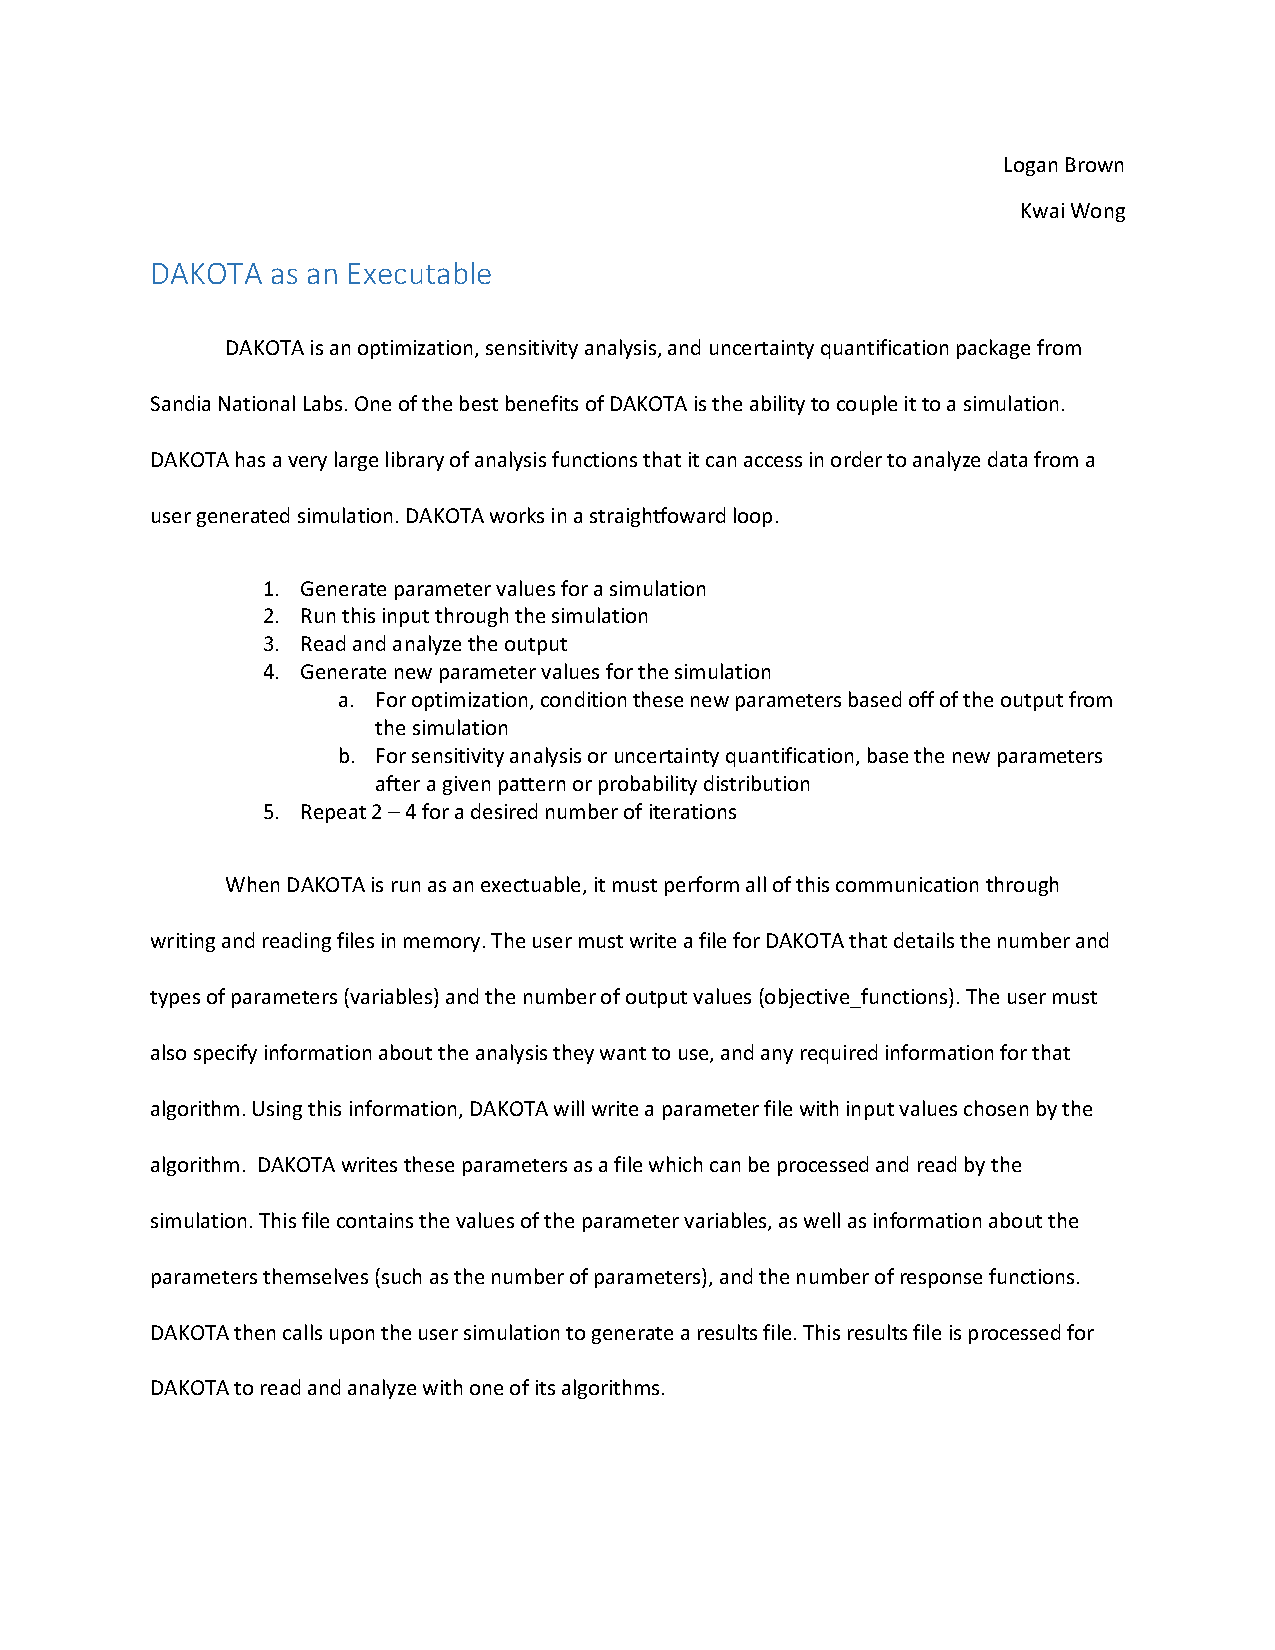
\includepdf[pages={1-7}]{extraFiles/DakotaLibrary_03-07-2014.pdf}

\end{document}
